\documentclass[12pt,a4paper,oneside]{article}\usepackage[]{graphicx}\usepackage[]{color}
%% maxwidth is the original width if it is less than linewidth
%% otherwise use linewidth (to make sure the graphics do not exceed the margin)
\makeatletter
\def\maxwidth{ %
  \ifdim\Gin@nat@width>\linewidth
    \linewidth
  \else
    \Gin@nat@width
  \fi
}
\makeatother

\definecolor{fgcolor}{rgb}{0.345, 0.345, 0.345}
\newcommand{\hlnum}[1]{\textcolor[rgb]{0.686,0.059,0.569}{#1}}%
\newcommand{\hlstr}[1]{\textcolor[rgb]{0.192,0.494,0.8}{#1}}%
\newcommand{\hlcom}[1]{\textcolor[rgb]{0.678,0.584,0.686}{\textit{#1}}}%
\newcommand{\hlopt}[1]{\textcolor[rgb]{0,0,0}{#1}}%
\newcommand{\hlstd}[1]{\textcolor[rgb]{0.345,0.345,0.345}{#1}}%
\newcommand{\hlkwa}[1]{\textcolor[rgb]{0.161,0.373,0.58}{\textbf{#1}}}%
\newcommand{\hlkwb}[1]{\textcolor[rgb]{0.69,0.353,0.396}{#1}}%
\newcommand{\hlkwc}[1]{\textcolor[rgb]{0.333,0.667,0.333}{#1}}%
\newcommand{\hlkwd}[1]{\textcolor[rgb]{0.737,0.353,0.396}{\textbf{#1}}}%

\usepackage{framed}
\makeatletter
\newenvironment{kframe}{%
 \def\at@end@of@kframe{}%
 \ifinner\ifhmode%
  \def\at@end@of@kframe{\end{minipage}}%
  \begin{minipage}{\columnwidth}%
 \fi\fi%
 \def\FrameCommand##1{\hskip\@totalleftmargin \hskip-\fboxsep
 \colorbox{shadecolor}{##1}\hskip-\fboxsep
     % There is no \\@totalrightmargin, so:
     \hskip-\linewidth \hskip-\@totalleftmargin \hskip\columnwidth}%
 \MakeFramed {\advance\hsize-\width
   \@totalleftmargin\z@ \linewidth\hsize
   \@setminipage}}%
 {\par\unskip\endMakeFramed%
 \at@end@of@kframe}
\makeatother

\definecolor{shadecolor}{rgb}{.97, .97, .97}
\definecolor{messagecolor}{rgb}{0, 0, 0}
\definecolor{warningcolor}{rgb}{1, 0, 1}
\definecolor{errorcolor}{rgb}{1, 0, 0}
\newenvironment{knitrout}{}{} % an empty environment to be redefined in TeX

\usepackage{alltt}
\usepackage[usenames,dvipsnames]{xcolor}
\usepackage{graphicx}
\usepackage{amsmath}
\usepackage{booktabs}
\setlength\parindent{0pt}



\IfFileExists{upquote.sty}{\usepackage{upquote}}{}
\begin{document}

\title{\color{TealBlue} cgmisc \\\ \normalsize Package containing various functions useful in computational genetics, especially in genome-wide association studies}
\author{\color{Orange}Marcin Kierczak}
\maketitle

\newpage

\section*{Introduction}
\subsection*{Synopsis}
\noindent Package cgmisc contains miscellaneous functions, hopefully useful for extending genome-wide association study (GWAS) analyses.

\subsection*{Purpose of this document}
\noindent This document aims at presenting how to use functions provided in the \texttt{cgmisc} package in a typical GWAS data analyses workflow. It is, however, not aiming to be a standalone GWAS tutorial as such.

\subsection*{Conventions}
Here, we present typographic conventions used throughout the text in order to facilitate following this document.
\begin{itemize}
\item{All R commands are written in terminal type: {\tt myfun(foo=T, bar=54)}}
\item{In the above example: \textit{myfun} is a function and both \textit{foo} and \textit{bar} are its arguments}
\end{itemize}

\subsection*{Getting help}
\noindent Like every other R function, the functions provided in this package are documented in the standard R-help (Rd) format and can be easily accessed by issuing \textbf{help}() or its shorter version, \textbf{?} function. For instance, if you want to get more information on how to use the clump.markers() function, type either \texttt{help(clumpmarkers)} or \texttt{?clump.markers} and press return/enter. To see this document from within R you type \texttt{vignette(`cgmisc`)}.

\section*{Working with \texttt{cgmisc}}
\subsection*{Installation}
\noindent In order to install \texttt{cgmisc}, you either use one of the R GUIs (native R GUI, RStudio etc.) or type the following command:

\begin{knitrout}\footnotesize
\definecolor{shadecolor}{rgb}{0.969, 0.969, 0.969}\color{fgcolor}\begin{kframe}
\begin{alltt}
 \hlkwd{install.packages}\hlstd{(}\hlstr{"cgmisc"}\hlstd{,} \hlkwc{repos}\hlstd{=}\hlstr{""}\hlstd{)}
\end{alltt}
\end{kframe}
\end{knitrout}

\noindent Functions in the \texttt{cgmisc} package often complement or use \texttt{GenABEL} package functions and data structures. \texttt{GenABEL} is an excellent and widely-used R package for performing genome-wide association studies and much more\dots Therefore \texttt{GenABEL} will be loaded automagically when loading cgmisc. You can load \texttt{cgmisc} package as follows:

\begin{knitrout}\footnotesize
\definecolor{shadecolor}{rgb}{0.969, 0.969, 0.969}\color{fgcolor}\begin{kframe}
\begin{alltt}
\hlkwd{require}\hlstd{(}\hlstr{"cgmisc"}\hlstd{)}
\end{alltt}
\end{kframe}
\end{knitrout}

\section*{Loading and preparing example data}
First, we load the data, in this case internal cgmisc data.
\begin{knitrout}\footnotesize
\definecolor{shadecolor}{rgb}{0.969, 0.969, 0.969}\color{fgcolor}\begin{kframe}
\begin{alltt}
\hlkwd{data}\hlstd{(cgmisc_data)}
\end{alltt}
\end{kframe}
\end{knitrout}
And run some quality checks. It is important not to exclude any markers due to their low minor allele frequency as we will be looking for stretches of homozygosity.
\begin{knitrout}\footnotesize
\definecolor{shadecolor}{rgb}{0.969, 0.969, 0.969}\color{fgcolor}\begin{kframe}
\begin{alltt}
\hlstd{qc} \hlkwb{<-} \hlkwd{check.marker}\hlstd{(data,} \hlkwc{callrate} \hlstd{=} \hlnum{0.95}\hlstd{,} \hlkwc{perid.call} \hlstd{=} \hlnum{0.95}\hlstd{,} \hlkwc{maf} \hlstd{=} \hlopt{-}\hlnum{1}\hlstd{)}
\hlstd{data.clean} \hlkwb{<-} \hlstd{data[qc}\hlopt{$}\hlstd{idok, qc}\hlopt{$}\hlstd{snpok]}
\end{alltt}
\end{kframe}
\end{knitrout}
Once data is clean and neat, we can look at genomic kinship and try to determine population structure:
\begin{knitrout}\footnotesize
\definecolor{shadecolor}{rgb}{0.969, 0.969, 0.969}\color{fgcolor}\begin{kframe}
\begin{alltt}
\hlstd{gkin} \hlkwb{<-} \hlkwd{ibs}\hlstd{(data.clean,} \hlkwc{weight} \hlstd{=} \hlstr{"freq"}\hlstd{)}
\hlstd{gkin.dist} \hlkwb{<-} \hlkwd{as.dist}\hlstd{(}\hlnum{0.5} \hlopt{-} \hlstd{gkin)}
\hlstd{gkin.mds} \hlkwb{<-} \hlkwd{cmdscale}\hlstd{(gkin.dist)}
\hlkwd{plot}\hlstd{(gkin.mds,} \hlkwc{xlab} \hlstd{=} \hlstr{"MDS1"}\hlstd{,} \hlkwc{ylab} \hlstd{=} \hlstr{"MDS2"}\hlstd{,} \hlkwc{las} \hlstd{=} \hlnum{1}\hlstd{,} \hlkwc{bty} \hlstd{=} \hlstr{"n"}\hlstd{)}
\hlkwd{grid}\hlstd{()}
\end{alltt}
\end{kframe}\begin{figure}[]


{\centering 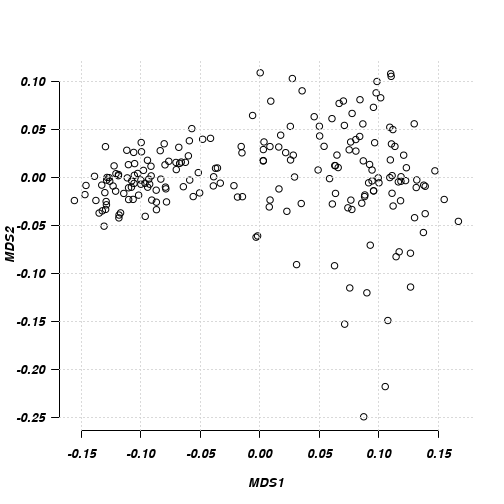
\includegraphics[width=1.0\textwidth]{images/gkin} 

}

\caption[An MDS projection of genomic kinship]{An MDS projection of genomic kinship.\label{fig:gkin}}
\end{figure}


\end{knitrout}
So, it seems there is some population structure in here. Just by eyeballing, we can spot two distinct clusters of individuals.\footnote{Well, OK, we actually did a scree test to see there is two clusters here. Eyeballing is not very scientific.} Let's run a simple k-means clustering to determine which individuals belong to which cluster.
\begin{knitrout}\footnotesize
\definecolor{shadecolor}{rgb}{0.969, 0.969, 0.969}\color{fgcolor}\begin{kframe}
\begin{alltt}
\hlstd{km} \hlkwb{<-} \hlkwd{kmeans}\hlstd{(gkin.mds,} \hlkwc{centers} \hlstd{=} \hlnum{2}\hlstd{)}
\hlstd{pop} \hlkwb{<-} \hlstd{km}\hlopt{$}\hlstd{cluster}
\hlkwd{plot}\hlstd{(gkin.mds,} \hlkwc{xlab} \hlstd{=} \hlstr{"MDS1"}\hlstd{,} \hlkwc{ylab} \hlstd{=} \hlstr{"MDS2"}\hlstd{,} \hlkwc{col} \hlstd{= pop,} \hlkwc{las} \hlstd{=} \hlnum{1}\hlstd{,} \hlkwc{bty} \hlstd{=} \hlstr{"n"}\hlstd{)}
\hlkwd{grid}\hlstd{()}
\end{alltt}
\end{kframe}\begin{figure}[]


{\centering 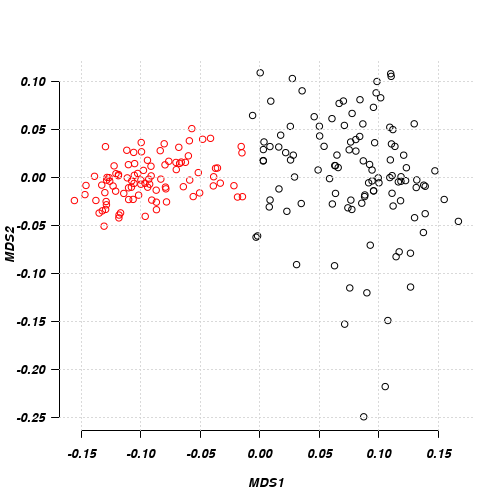
\includegraphics[width=1.0\textwidth]{images/gkin_pops} 

}

\caption[An MDS projection of genomic kinship]{An MDS projection of genomic kinship.\label{fig:gkin.pops}}
\end{figure}


\end{knitrout}
\section*{Comparing allele counts between populations}
To compare allele counts between two populations, you first need to call {\tt pop.allele.counts} function. You supply data (in our case only chromosome 27) and pop vector which assigns each individual to a population. Populations have to be encoded as 1 and 2. In addition, there is an option {\tt progress} which turns on and off displaying of the progress bar.
\begin{knitrout}\footnotesize
\definecolor{shadecolor}{rgb}{0.969, 0.969, 0.969}\color{fgcolor}\begin{kframe}
\begin{alltt}
\hlstd{dat} \hlkwb{<-} \hlstd{data.clean[, data.clean}\hlopt{@}\hlkwc{gtdata}\hlopt{@}\hlkwc{chromosome} \hlopt{==} \hlstr{"27"}\hlstd{]}
\hlstd{allele.counts} \hlkwb{<-} \hlkwd{pop.allele.counts}\hlstd{(}\hlkwc{data} \hlstd{= dat,} \hlkwc{pops} \hlstd{= pop,} \hlkwc{progress} \hlstd{= F)}
\end{alltt}
\end{kframe}
\end{knitrout}
Now, when the tests are finished, you may want to plot the result. If you are plotting single chromosome, you may want to turn on coloring markers by LD (still experimental option).
\begin{knitrout}\footnotesize
\definecolor{shadecolor}{rgb}{0.969, 0.969, 0.969}\color{fgcolor}\begin{kframe}
\begin{alltt}
\hlkwd{plot.pac}\hlstd{(}\hlkwc{data} \hlstd{= dat,} \hlkwc{allele.cnt} \hlstd{= allele.counts,} \hlkwc{plot.LD} \hlstd{= T)}
\end{alltt}


{\ttfamily\noindent\itshape\color{messagecolor}{\#\# Loading required package: wesanderson}}\end{kframe}

{\centering 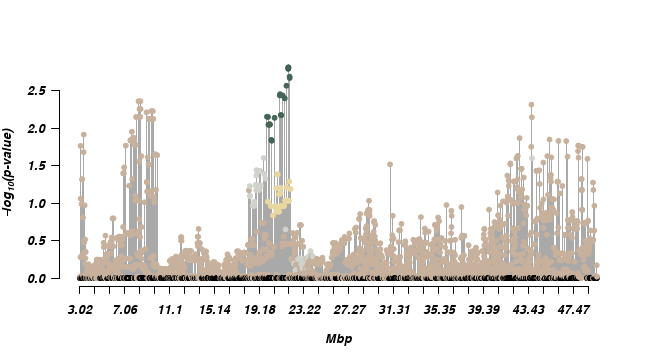
\includegraphics[width=1.0\textwidth]{images/plot_pac1} 

}



\end{knitrout}
But what if you want to plot the result in a custom way, say applying some window-based smoothing? The simplest type of window will be based on a number of markers, say we want to apply smoothing based on a sliding window of 21 markers:
\begin{knitrout}\footnotesize
\definecolor{shadecolor}{rgb}{0.969, 0.969, 0.969}\color{fgcolor}\begin{kframe}
\begin{alltt}
\hlstd{coords} \hlkwb{<-} \hlstd{allele.counts}\hlopt{@}\hlkwc{map}
\hlstd{p.vals} \hlkwb{<-} \hlopt{-}\hlkwd{log10}\hlstd{(allele.counts}\hlopt{@}\hlkwc{p.values}\hlstd{)}
\hlcom{# Handle NAs for the nice look}
\hlstd{p.vals[}\hlkwd{is.na}\hlstd{(p.vals)]} \hlkwb{<-} \hlnum{0}
\hlstd{filter21} \hlkwb{<-} \hlkwd{rep}\hlstd{(}\hlnum{1}\hlopt{/}\hlnum{21}\hlstd{,} \hlnum{21}\hlstd{)}
\hlstd{smooth} \hlkwb{<-} \hlkwd{filter}\hlstd{(p.vals, filter21,} \hlkwc{sides}\hlstd{=}\hlnum{2}\hlstd{)}
\hlkwd{plot}\hlstd{(coords}\hlopt{/}\hlnum{1e6}\hlstd{, p.vals,} \hlkwc{xlab}\hlstd{=}\hlstr{"Mb"}\hlstd{,} \hlkwc{type}\hlstd{=}\hlstr{'l'}\hlstd{,} \hlkwc{col}\hlstd{=}\hlstr{"grey"}\hlstd{,}
     \hlkwc{bty}\hlstd{=}\hlstr{'n'}\hlstd{,} \hlkwc{xlim}\hlstd{=}\hlkwd{c}\hlstd{(}\hlnum{0}\hlstd{,}\hlnum{50}\hlstd{),} \hlkwc{las}\hlstd{=}\hlnum{1}\hlstd{)}
\hlkwd{lines}\hlstd{(coords}\hlopt{/}\hlnum{1e6}\hlstd{, smooth,} \hlkwc{col}\hlstd{=}\hlstr{'blue'}\hlstd{)}
\hlkwd{grid}\hlstd{()}
\end{alltt}
\end{kframe}

{\centering 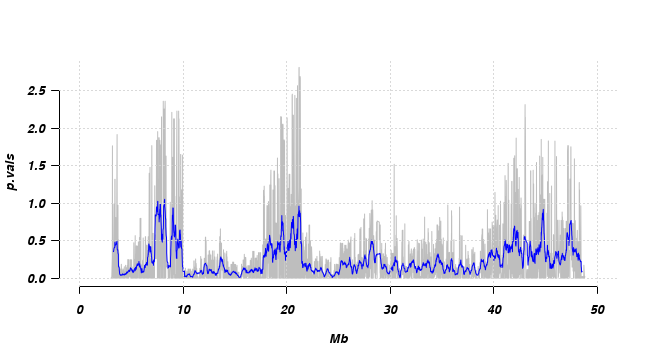
\includegraphics[width=1.0\textwidth]{images/plot_pac_smooth} 

}



\end{knitrout}
And what if you want the windows to span certain number of base pairs?
\begin{knitrout}\footnotesize
\definecolor{shadecolor}{rgb}{0.969, 0.969, 0.969}\color{fgcolor}\begin{kframe}
\begin{alltt}
\hlcom{# Prepare a matrix of overlapping windows}
\hlstd{W} \hlkwb{<-} \hlkwd{get.overlapping.windows}\hlstd{(}\hlkwc{data} \hlstd{= dat,} \hlkwc{chr} \hlstd{=} \hlnum{27}\hlstd{,} \hlkwc{size} \hlstd{=} \hlnum{1e6}\hlstd{,}
                             \hlkwc{overlap} \hlstd{=} \hlnum{25e4}\hlstd{)}
\hlcom{# Get mean values per window}
\hlstd{PW} \hlkwb{<-} \hlkwd{apply}\hlstd{(W[[}\hlnum{2}\hlstd{]],} \hlkwc{MARGIN} \hlstd{=} \hlnum{1}\hlstd{,} \hlkwc{FUN} \hlstd{=} \hlkwa{function}\hlstd{(}\hlkwc{x}\hlstd{) \{} \hlkwd{mean}\hlstd{(x} \hlopt{*} \hlstd{p.vals) \} )}
\hlcom{# Do plotting }
\hlkwd{plot}\hlstd{(W[[}\hlnum{1}\hlstd{]]}\hlopt{$}\hlstd{midpoint}\hlopt{/}\hlnum{1e6}\hlstd{, PW,} \hlkwc{type}\hlstd{=}\hlstr{'h'}\hlstd{,}
    \hlkwc{col}\hlstd{=}\hlkwd{wes.palette}\hlstd{(}\hlnum{2}\hlstd{,}\hlkwc{name} \hlstd{=} \hlstr{"Cavalcanti"}\hlstd{)[}\hlnum{1}\hlstd{],}
    \hlkwc{xlim}\hlstd{=}\hlkwd{c}\hlstd{(}\hlnum{0}\hlstd{,}\hlnum{50}\hlstd{),}
    \hlkwc{las}\hlstd{=}\hlnum{1}\hlstd{,} \hlkwc{bty}\hlstd{=}\hlstr{'n'}\hlstd{,} \hlkwc{xlab}\hlstd{=}\hlstr{"Mb"}\hlstd{,} \hlkwc{ylab}\hlstd{=}\hlstr{"Mean -log10(p-value)"}\hlstd{)}
\hlkwd{grid}\hlstd{()}
\end{alltt}
\end{kframe}

{\centering 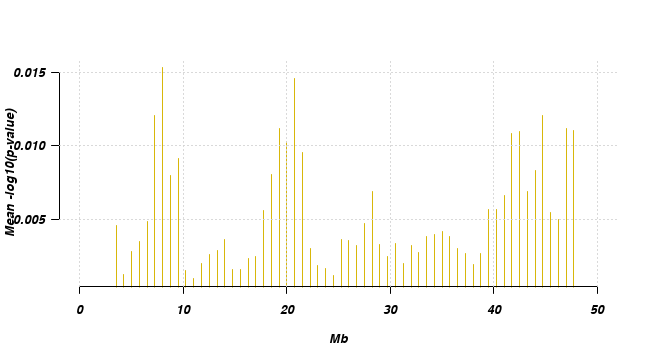
\includegraphics[width=1.0\textwidth]{images/pac_plot_smooth2} 

}



\end{knitrout}
It is also quite common to discard windows which contain just a few markers. Here, we set the threshold to 65 markers in a window. It is probably way too high, but we do it just as an example of how one can do filtering.
\begin{knitrout}\footnotesize
\definecolor{shadecolor}{rgb}{0.969, 0.969, 0.969}\color{fgcolor}\begin{kframe}
\begin{alltt}
\hlstd{window.len} \hlkwb{<-} \hlkwd{apply}\hlstd{(W[[}\hlnum{2}\hlstd{]],} \hlkwc{MARGIN} \hlstd{=} \hlnum{1}\hlstd{, sum)}
\hlstd{threshold} \hlkwb{<-} \hlnum{65}
\hlstd{W.filtered} \hlkwb{<-} \hlkwd{list}\hlstd{(W[[}\hlnum{1}\hlstd{]][window.len} \hlopt{>=} \hlstd{threshold,],}
                   \hlstd{W[[}\hlnum{2}\hlstd{]][window.len} \hlopt{>=} \hlstd{threshold,])}
\hlstd{PW.filtered} \hlkwb{<-} \hlkwd{apply}\hlstd{(W.filtered[[}\hlnum{2}\hlstd{]],}
                     \hlkwc{MARGIN} \hlstd{=} \hlnum{1}\hlstd{,}
                     \hlkwc{FUN} \hlstd{=} \hlkwa{function}\hlstd{(}\hlkwc{x}\hlstd{) \{} \hlkwd{mean}\hlstd{(x} \hlopt{*} \hlstd{p.vals) \} )}
\hlkwd{plot}\hlstd{(W.filtered[[}\hlnum{1}\hlstd{]]}\hlopt{$}\hlstd{midpoint}\hlopt{/}\hlnum{1e6}\hlstd{, PW.filtered,} \hlkwc{type}\hlstd{=}\hlstr{'h'}\hlstd{,}
    \hlkwc{col}\hlstd{=}\hlkwd{wes.palette}\hlstd{(}\hlnum{2}\hlstd{,}\hlkwc{name} \hlstd{=} \hlstr{"Cavalcanti"}\hlstd{)[}\hlnum{1}\hlstd{],}
    \hlkwc{xlim}\hlstd{=}\hlkwd{c}\hlstd{(}\hlnum{0}\hlstd{,}\hlnum{50}\hlstd{),}
    \hlkwc{las}\hlstd{=}\hlnum{1}\hlstd{,} \hlkwc{bty}\hlstd{=}\hlstr{'n'}\hlstd{,} \hlkwc{xlab}\hlstd{=}\hlstr{"Mb"}\hlstd{,} \hlkwc{ylab}\hlstd{=}\hlstr{"Mean -log10(p-value)"}\hlstd{)}
\hlkwd{grid}\hlstd{()}
\end{alltt}
\end{kframe}

{\centering 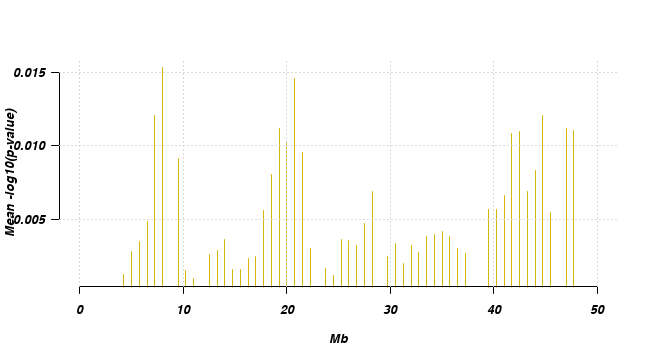
\includegraphics[width=1.0\textwidth]{images/pac_plot_filtered_windows} 

}



\end{knitrout}

\subsection*{Computing and plotting $F_{ST}$}
The fixation index ($F_{ST}$) is a widely used measure of population differentiation due to genetic structure. \texttt{cgmisc} package provides a function \texttt{compute.Fstats} that, along with \texttt{plot.Fstats} function, enable computation and visualization of $F_{ST}$ for a pair of populations.
\begin{knitrout}\footnotesize
\definecolor{shadecolor}{rgb}{0.969, 0.969, 0.969}\color{fgcolor}\begin{kframe}
\begin{alltt}
\hlstd{fst} \hlkwb{<-} \hlkwd{compute.Fstats}\hlstd{(}\hlkwc{data} \hlstd{= dat,} \hlkwc{pops} \hlstd{= pop)}
\hlkwd{plot.fstats}\hlstd{(}\hlkwc{data} \hlstd{= dat,} \hlkwc{fstats} \hlstd{= fst)}
\end{alltt}
\end{kframe}

{\centering 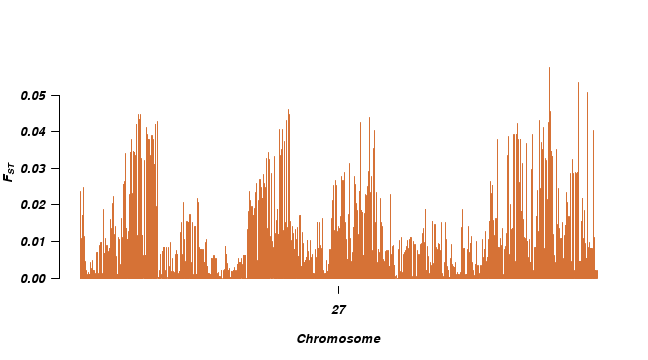
\includegraphics[width=1.0\textwidth]{images/fst} 

}



\end{knitrout}
The \texttt{computeFstats} function returns an object of \texttt{fstats.result} class which contains two \textit{slots}: global statistics, statistics for populations. Global statistics is a \textit{data frame} and can be accessed by using either \texttt{glob(fst)} or \texttt{fst@glob} notation. Let's try to see global statistics for the 5 first markers:
\begin{knitrout}\footnotesize
\definecolor{shadecolor}{rgb}{0.969, 0.969, 0.969}\color{fgcolor}\begin{kframe}
\begin{alltt}
\hlstd{fst}\hlopt{@}\hlkwc{glob}\hlstd{[}\hlnum{1}\hlopt{:}\hlnum{5}\hlstd{, ]}
\end{alltt}
\begin{verbatim}
##    p.bar    q.bar       HI       HS       HT       FIS      FST       FIT
## 1 1.0000 0.000000 0.000000 0.000000 0.000000       NaN      NaN       NaN
## 2 1.0000 0.000000 0.000000 0.000000 0.000000       NaN      NaN       NaN
## 3 0.9975 0.002463 0.004926 0.004909 0.004914 -0.003517 0.001044 -0.002469
## 4 1.0000 0.000000 0.000000 0.000000 0.000000       NaN      NaN       NaN
## 5 0.9951 0.004926 0.009852 0.009783 0.009804 -0.007058 0.002093 -0.004950
\end{verbatim}
\end{kframe}
\end{knitrout}
Here, we can see 8 different columns for every marker. The meaning of these is:
\begin{itemize}
  \item{p.bar and q.bar -- allele frequencies based on all individuals},
  \item{HI, HS and HT -- global heterozygosity indices based on the observed allele frequencies, allele frequencies expected under the \textit{null} and allele frequencies computed using all individuals, respectively.}
  \item{FIS, FST and FIT -- inbreeding coefficient individual/subpopulation ($F_{IS}$), subpopulation effect ($F_{ST}$) and inbreeding coefficient individual/total population ($F_{IT}$)}
\end{itemize}
Now, let us examine statistics obtained for the first 5 markers in subpopulation 2:
\begin{knitrout}\footnotesize
\definecolor{shadecolor}{rgb}{0.969, 0.969, 0.969}\color{fgcolor}\begin{kframe}
\begin{alltt}
\hlstd{fst}\hlopt{@}\hlkwc{pops}\hlstd{[[}\hlnum{2}\hlstd{]][}\hlnum{1}\hlopt{:}\hlnum{5}\hlstd{, ]}
\end{alltt}
\begin{verbatim}
##                AA Aa aa   N      p        q exp.AA exp.Aa   exp.aa
## TIGRP2P347125 110  0  0 110 1.0000 0.000000    110 0.0000 0.000000
## BICF2P1061825 110  0  0 110 1.0000 0.000000    110 0.0000 0.000000
## BICF2P522661  109  1  0 110 0.9955 0.004545    109 0.9955 0.002273
## BICF2P577353  110  0  0 110 1.0000 0.000000    110 0.0000 0.000000
## BICF2P467643  108  2  0 110 0.9909 0.009091    108 1.9818 0.009091
##                obs.het exp.het    dev.het        Fs
## TIGRP2P347125 0.000000 0.00000  0.000e+00       NaN
## BICF2P1061825 0.000000 0.00000  0.000e+00       NaN
## BICF2P522661  0.009091 0.00905 -4.132e-05 -0.004566
## BICF2P577353  0.000000 0.00000  0.000e+00       NaN
## BICF2P467643  0.018182 0.01802 -1.653e-04 -0.009174
\end{verbatim}
\end{kframe}
\end{knitrout}
Here, we have the following columns per each marker: 
\begin{itemize}
  \item{AA, Aa and aa -- observed genotype counts,}
  \item{p, q -- observed allele frequencies,}
  \item{exp.AA, exp.Aa, exp.aa -- genotype frequencies expected under the \textit{null},}
  \item{obs.het, exp.het, dev.het -- observed heterozygosity, heterozygosity expected under the \textit{null} and difference of the two above,}
  \item{Fs -- F-statistics value}
\end{itemize}

\section*{Visualizing LD-decay}
To visualize average rate of LD-decay with the distance between markers, one can use the \texttt{plot.LD.decay} function. It lets one specify the minimal and the maximal distance considered as well as the number of bins used in binning LD values. The more bins, the more ``jumpy'' the curve will be, the less bins the ``smoother'' the curve but at the same time the lower resolution. So choose something aroud 100 bins as a good compromise.
\begin{knitrout}\footnotesize
\definecolor{shadecolor}{rgb}{0.969, 0.969, 0.969}\color{fgcolor}\begin{kframe}
\begin{alltt}
\hlkwd{plot.LD.decay}\hlstd{(}\hlkwc{data}\hlstd{=dat,} \hlkwc{N}\hlstd{=}\hlnum{100}\hlstd{,} \hlkwc{dmin}\hlstd{=}\hlnum{0}\hlstd{,} \hlkwc{dmax}\hlstd{=}\hlnum{1e6}\hlstd{,}
              \hlkwc{main}\hlstd{=}\hlstr{"LD decay on chr 27"}\hlstd{)}
\end{alltt}
\end{kframe}

{\centering 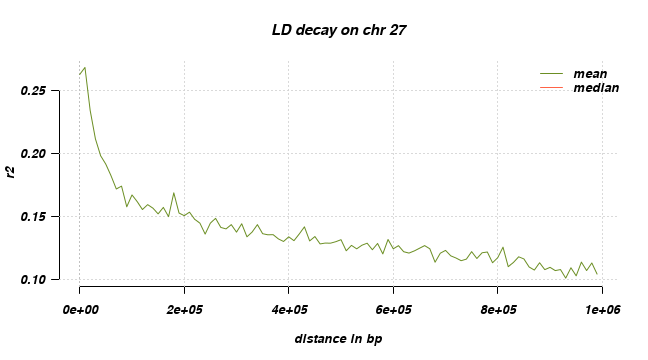
\includegraphics[width=1.0\textwidth]{images/ld_decay} 

}



\end{knitrout}

\section*{Endogenous retroviral sequences}
Given a set of coordinates in canFam3, returns $-log(p-value)$ of hits reflecting the likelihood that a particular region is an endogenous retroviral sequence (ERV). 
\begin{knitrout}\footnotesize
\definecolor{shadecolor}{rgb}{0.969, 0.969, 0.969}\color{fgcolor}\begin{kframe}
\begin{alltt}
\hlkwd{plot.erv}\hlstd{(}\hlstr{"chr16"}\hlstd{,} \hlkwc{coords} \hlstd{=} \hlkwd{c}\hlstd{(}\hlnum{1500000}\hlstd{,} \hlnum{1700000}\hlstd{))}
\end{alltt}
\end{kframe}

{\centering 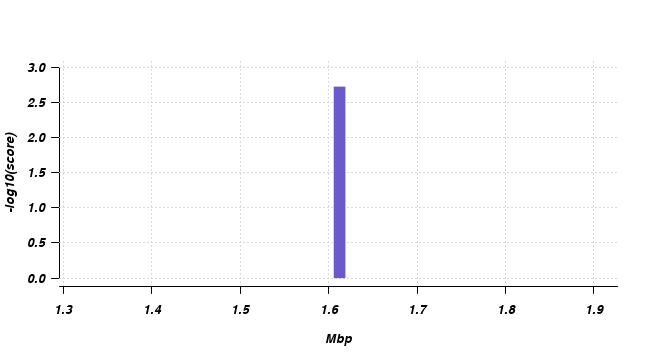
\includegraphics[width=1.0\textwidth]{images/plot_ervs} 

}



\end{knitrout}

\section*{Association Analysis}
\noindent Some of \texttt{cgmisc} functions use data which are the result of GWAS analyses. Let's perform GWAS on our data to obtain \texttt{GenABEL} \texttt{scan.gwaa-class} object : 

\begin{knitrout}\footnotesize
\definecolor{shadecolor}{rgb}{0.969, 0.969, 0.969}\color{fgcolor}\begin{kframe}
\begin{alltt}
\hlstd{an0} \hlkwb{<-} \hlkwd{qtscore}\hlstd{(response} \hlopt{~} \hlstd{sex,} \hlkwc{data} \hlstd{= data)}
\end{alltt}


{\ttfamily\noindent\color{warningcolor}{\#\# Warning: 1 observations deleted due to missingness}}\end{kframe}
\end{knitrout}

\noindent And have a look at top 5 markers

\begin{knitrout}\footnotesize
\definecolor{shadecolor}{rgb}{0.969, 0.969, 0.969}\color{fgcolor}\begin{kframe}
\begin{alltt}
\hlkwd{summary}\hlstd{(an0,} \hlkwc{top} \hlstd{=} \hlnum{5}\hlstd{)}
\end{alltt}
\begin{verbatim}
## Summary for top 5 results, sorted by P1df
##                 Chromosome Position Strand A1 A2   N    effB se_effB
## BICF2P1063345           34 40399702      u  T  G 206 -0.2834 0.06954
## BICF2P682714             1 15399848      u  A  G 189  0.5887 0.14714
## BICF2G630569243          6 80458945      u  C  A 206  0.3071 0.07797
## BICF2S2366791            6 70667322      u  C  T 206  0.2628 0.06682
## BICF2G630450144         34 40416964      u  A  G 206 -0.2705 0.06933
##                 chi2.1df      P1df   effAB   effBB chi2.2df      P2df
## BICF2P1063345      16.60 4.609e-05 -0.3644 -0.5354    17.51 1.579e-04
## BICF2P682714       16.01 6.309e-05  0.5912  1.1515    16.01 3.339e-04
## BICF2G630569243    15.51 8.216e-05  0.2904  0.6358    15.57 4.167e-04
## BICF2S2366791      15.46 8.410e-05  0.4558  0.4732    20.15 4.202e-05
## BICF2G630450144    15.22 9.573e-05 -0.3339 -0.5161    15.77 3.756e-04
##                     Pc1df
## BICF2P1063345   7.357e-05
## BICF2P682714    9.911e-05
## BICF2G630569243 1.274e-04
## BICF2S2366791   1.302e-04
## BICF2G630450144 1.472e-04
\end{verbatim}
\end{kframe}
\end{knitrout}

\subsection*{Plotting qunatile-quantile plot of p-values}
\begin{knitrout}\footnotesize
\definecolor{shadecolor}{rgb}{0.969, 0.969, 0.969}\color{fgcolor}\begin{kframe}
\begin{alltt}
\hlkwd{plot.qq}\hlstd{(}\hlkwc{pvals} \hlstd{= an0}\hlopt{@}\hlkwc{results}\hlopt{$}\hlstd{P1df,} \hlkwc{conf} \hlstd{=} \hlkwd{c}\hlstd{(}\hlnum{0.05}\hlstd{,} \hlnum{0.95}\hlstd{),} \hlkwc{step} \hlstd{=} \hlnum{100}\hlstd{)}
\end{alltt}
\end{kframe}

{\centering 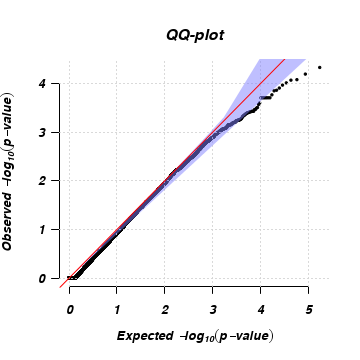
\includegraphics[width=1.0\textwidth]{images/plot_qq} 

}



\end{knitrout}

\subsection*{Plot.Manhattan.LD}
\noindent The \texttt{plot.Manhattan.LD} function allows you to visualize the LD pattern in a genome fragment on an enchanced Manhattan plot. You select one marker, typically the one with the strongest association to the analysed trait and all other markers in the region are coloured according to the degree of linkage disequilibrium with this index marker. 

\begin{knitrout}\footnotesize
\definecolor{shadecolor}{rgb}{0.969, 0.969, 0.969}\color{fgcolor}\begin{kframe}
\begin{alltt}
\hlkwd{plot.manhattan.LD}\hlstd{(data, an0,} \hlkwc{chr}\hlstd{=}\hlnum{34}\hlstd{,} \hlkwc{region}\hlstd{=}\hlkwd{c}\hlstd{(}\hlnum{39e6}\hlstd{,}\hlnum{42e6}\hlstd{),}
                  \hlkwc{index.snp} \hlstd{=} \hlstr{'BICF2P1063345'}\hlstd{,} \hlkwc{bonferroni} \hlstd{= F)}
\end{alltt}
\end{kframe}

{\centering 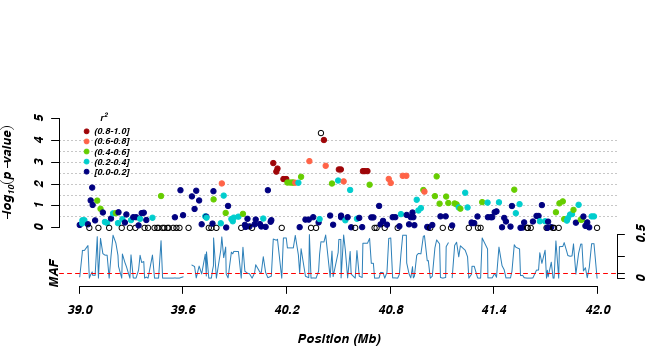
\includegraphics[width=1.0\textwidth]{images/plot_Manhattan_LD} 

}



\end{knitrout}

\subsection*{Clumping}
\noindent \texttt{clump.markers} function implements clumping procedure described in PLINK documentation. Clumping is based on linkage disequilibrium. The function returns list of clumps which can be used for further analyses or plotted using \texttt{plot.clumps} function included in our package.

\begin{knitrout}\footnotesize
\definecolor{shadecolor}{rgb}{0.969, 0.969, 0.969}\color{fgcolor}\begin{kframe}
\begin{alltt}
\hlstd{clumps} \hlkwb{<-} \hlkwd{clump.markers}\hlstd{(data,} \hlkwc{gwas.result} \hlstd{= an0,} \hlkwc{chr} \hlstd{=} \hlnum{6}\hlstd{,} \hlkwc{bp.dist} \hlstd{=} \hlnum{250000}\hlstd{,}
    \hlkwc{p1} \hlstd{=} \hlnum{1e-04}\hlstd{,} \hlkwc{p2} \hlstd{=} \hlnum{0.01}\hlstd{,} \hlkwc{r2} \hlstd{=} \hlnum{0.5}\hlstd{,} \hlkwc{image} \hlstd{= T)}
\end{alltt}
\end{kframe}

{\centering 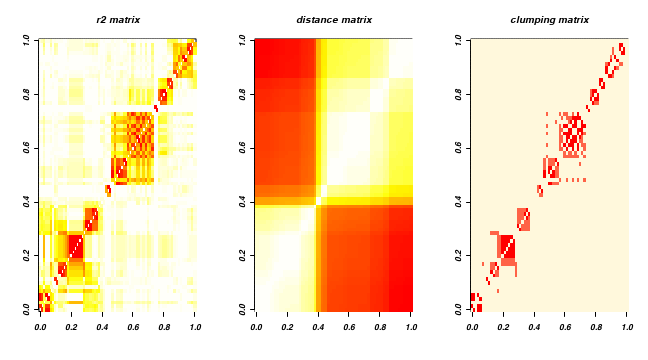
\includegraphics[width=1.0\textwidth]{images/clump_markers} 

}



\end{knitrout}

Now, one can plot clumps using the \texttt{plot.clumps()} function:
\begin{knitrout}\footnotesize
\definecolor{shadecolor}{rgb}{0.969, 0.969, 0.969}\color{fgcolor}\begin{kframe}
\begin{alltt}
\hlkwd{plot.clumps}\hlstd{(}\hlkwc{gwas.result} \hlstd{= an0,} \hlkwc{clumps} \hlstd{= clumps,}
            \hlkwc{chr} \hlstd{=} \hlnum{6}\hlstd{,} \hlkwc{region} \hlstd{=} \hlkwd{c}\hlstd{(}\hlnum{68.3e6}\hlstd{,} \hlnum{81.6e6}\hlstd{))}
\end{alltt}
\end{kframe}

{\centering 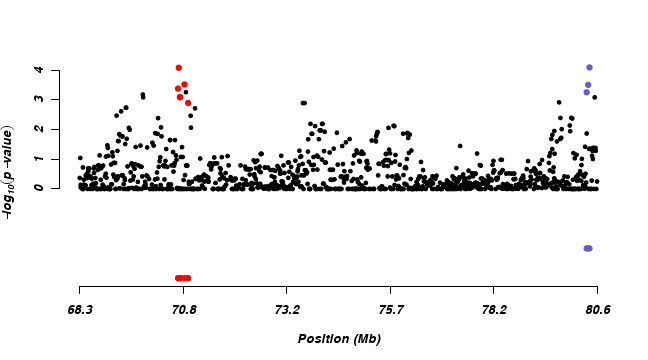
\includegraphics[width=1.0\textwidth]{images/plot_clumps} 

}



\end{knitrout}

\section*{Data conversion functions}
\subsection*{gwaa2bed}
\subsection*{gwaa2bigRR}
\subsection*{gwaa2PHASE}
\subsection*{gwaa2vgwas}
\subsection*{phase2fasta}
\subsection*{phase2haploview}

\section*{Convenience functions}
\subsection*{open.region.UCSC}
\subsection*{get.overlapping.windows}
\subsection*{get.erv}
\subsection*{get.adjacent.markers}
\subsection*{get.chr.midpoints}
\subsection*{get.LD.colors.r}
\subsection*{create.haploview.info}
\subsection*{choose.top.snps}

\section*{Species-specific functions}
\subsection*{Xfix.canfam}
\end{document}
